%! suppress = MissingImport
%! Author = maxwe
%! Date = 10.03.22

% Preamble
\documentclass[11pt]{PyRollDocs}

\addbibresource{refs.bib}

\newmintinline[py]{python}{}

% Document
\begin{document}

    \title{The Ring Model PyRoll Plugin}
    \author{Max Weiner}
    \date{\today}

    \maketitle

    The Ring Model plugin serves as a base package for other plugin using an 1D finite differences approach for modelling inhomogeneous workpiece state.


    \section{Model approach}\label{sec:model-approach}

    \begin{figure}
        \centering
        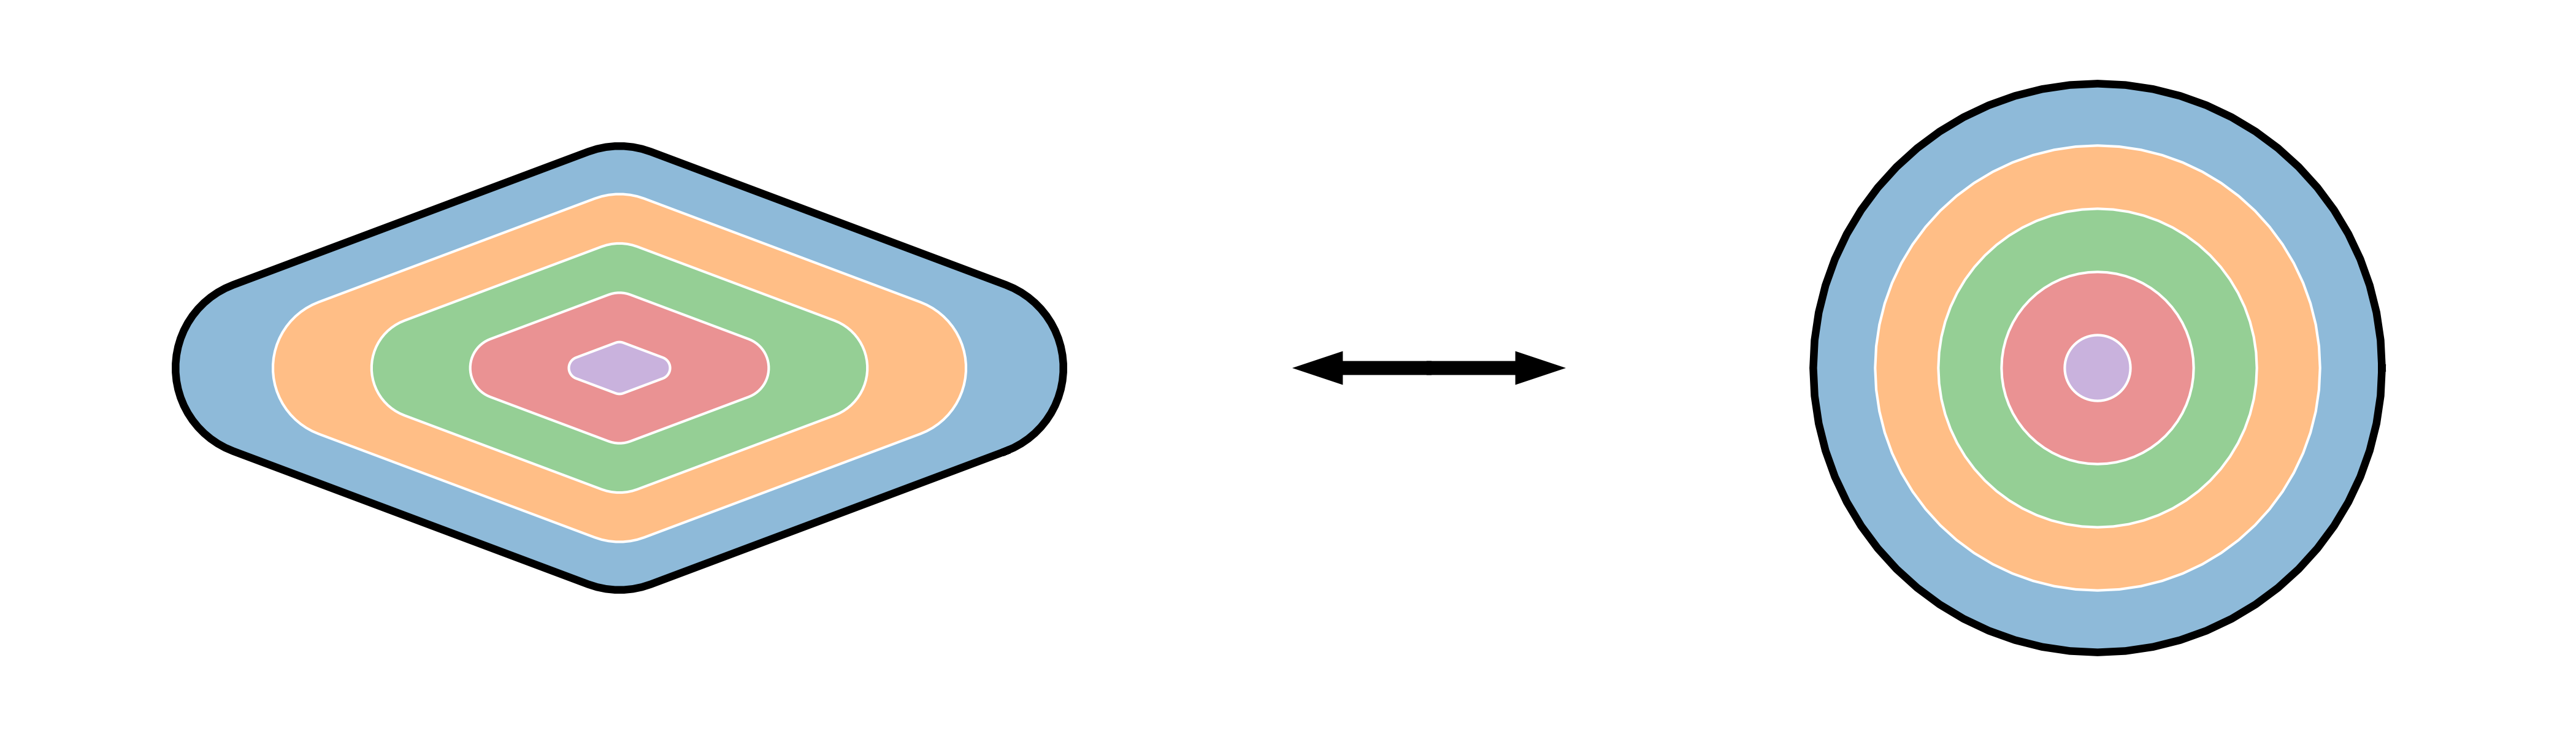
\includegraphics[width=\linewidth]{img/ring_model}
        \caption{Example of Ring Discretization for an Diamond Profile and its Equivalent Round Profile}
        \label{fig:ring_model}
    \end{figure}

    The ring model introduces a gradient in radial direction from core to surface of the profile while neglecting gradients in angular direction.
    The actual profile cross-section is mapped to an equivalent round profile, which is divided in concentric rings, as illustrated in \autoref{fig:ring_model}.
    In the implementation provided the equivalent radius $r_\mathrm{e}$ is defined by \autoref{eq:equivalent_radius} with the profile cross-section area $A$.

    \begin{equation}
        r_{\mathrm{e}} = \sqrt{\frac{A}{\pi}}
        \label{eq:equivalent_radius}
    \end{equation}

    The equivalent round is divided in equidistant concentric rings.
    The ring distance is $\Delta r$.
    The core ring is a circle with center in $(0,0)$ and radius $\frac{\Delta r}{2}$.
    Therefore, $\Delta r$ is calculated as in \autoref{eq:delta_r} with the count of rings $n$.

    \begin{equation}
        \Delta r = \frac{r_{\mathrm{e}}}{n - \frac{1}{2}}
        \label{eq:delta_r}
    \end{equation}

    The ring center lines' radii are as in \autoref{eq:ring_center} with the index of the ring $i \in [0, n-1]$.

    \begin{equation}
        r_i = i \Delta r
        \label{eq:ring_center}
    \end{equation}

    The radii of the ring boundary lines are as in \autoref{eq:ring_boundaries} with the index of the boundary $j \in [0, n]$.

    \begin{subequations}
        \begin{align}
            R_j &= \left(j - \frac{1}{2}\right) \Delta r\\
            R_0 &= 0
        \end{align}
        \label{eq:ring_boundaries}
    \end{subequations}

    The rings are mapped back to the actual cross-section by scaling the polar coordinates of the contour with the ring radii as in \autoref{eq:map_back}, with the polar coordinates of the profile contour line $(\theta, \varrho)$. $r_{\mathrm{P}i}(\theta)$ are the polar coordinates of the ring center lines on the actual profile cross-section like illustrated on the left of \autoref{fig:ring_model}.
    The boundaries' coordinates are calculated accordingly.

    \begin{subequations}
        \begin{gather}
            r_{\mathrm{P}i}(\theta) = \varrho(\theta) \frac{r_i}{r_{\mathrm{e}}}\\
            R_{\mathrm{P}j}(\theta) = \varrho(\theta) \frac{R_j}{r_{\mathrm{e}}}
        \end{gather}
        \label{eq:map_back}
    \end{subequations}

    The length of the mapped boundary lines is defined as the interface length $I_j$.
    The area between the mapped boundaries is the ring cross-section $A_i$.


    \section{Usage instructions}\label{sec:usage-instructions}

    Packages residing on this type of discretization shall depend on this plugin to create a common interface.
    In the following, the hooks defined by this plugin shall be described, and instructions shall be given, how to implement model equation for specific purposes.

    The ring model plugin only defines hooks on \py/pyroll.core.Profile/.
    The central hook of this package is \py/Profile.rings/.
    It returns a numpy array of radius coordinates representing the centers of the rings acc.\ to \autoref{eq:ring_center}.
    The respective ring boundaries' coordinates acc.\ to \autoref{eq:ring_boundaries}  are provided by the \py/Profile.ring_boundaries/ hook.
    The outermost boundary equals the equivalent radius acc.\ to \autoref{eq:equivalent_radius}  of the profile cross-section, which is also available from the \py/Profile.equivalent_radius/ hook.
    To modify the calculation of the equivalent radius, provide a new implementation of the \py/Profile.equivalent_radius/ hook.
    To modify the ring distancing, both \py/Profile.rings/ and \py/Profile.ring_boundaries/ should be provided.
    Users of this plugin should not rely on equidistant rings, but calculate needed distances from the respective coordinates.

    For geometric calculations, also two hooks returning shapely geometry objects are provided.
    \py/Profile.ring_contours/ returns an array of \py/LineStrings/ representing the mapping of the ring boundaries on the real profile cross-section.
    The interface lengths $I_j$ can be obtained by using \py/Profile.ring_contours[j].length/.
    \py/Profile.ring_sections/ returns, however, an array of \py/Polygon/ objects representing the areas of the rings lying between those boundaries.
    The ring cross-sections $A_i$ can be obtained by using \py/Profile.ring_sections[i].area/.

    For implementing model equations, define a new hook \py/Profile.ring_*s/ which shall return an array of the same length as \py/Profile.rings/.
    The \texttt{*} shall be replaced with the property name you want to represent, pay respect to the plural form.
    Ideally a hook named accordingly exists on \py/Profile/ or is defined alongside, which returns a mean value of the inhomogeneous data.
    For example the core hook \py/Profile.temperature/ may be accompanied by \py/Profile.ring_temperatures/ to hold inhomogeneous temperature data.

    \printbibliography

\end{document}